%---------- Inleiding ---------------------------------------------------------

\section{Introductie}%
\label{sec:introductie}

% TODO Bron voor de groei van python-pakketten toevoegen
België is een koploper in het gebruik van artificiële intelligentie (AI) op de werkvloer. Jaarlijks investeert de Vlaamse overheid 32 miljoen in het vakgebied \autocite{Crevits2022}. Zo zijn er verschillende projecten uit de grond gestampt om taalgerelateerde AI-ontwikkelingen op te starten. Vooral het amai!-project \footnote{https://amai.vlaanderen/} geeft de aanzet door twee toepassingen te ontwikkelen die nu in middelbare klassen terug te vinden zijn, namelijk \textit{real-time} ondertiteling en een taalassistent voor leerkrachten bij meertalige klasgroepen.

Het STEM-agenda\footnote{https://www.vlaanderen.be/publicaties/stem-agenda-2030-stem-competenties-voor-een-toekomst-en-missiegericht-beleid}
van de Vlaamse Overheid omvat aandachtspunten om het STEM-onderwijs tegen 2030 aantrekkelijker te maken door leraren, opleiders en begeleiders te ondersteunen. Het overbruggen van wetenschappelijke jargon is nergens in de aandachtspunten terug te vinden. Dit is echter spijtig, want de derde graad van het middelbaar onderwijs is een cruciale stap voor de verdere loopbaan van scholieren. 

Dit onderzoek achterhaalt welke toepassing het meest conform is aan de noden van een scholier met dyslexie in het derde graad middelbaar onderwijs bij het lezen van wetenschappelijke papers. Eerst vat het onderzoek samen wat tekstsimplificatie inhoudt en uit welke soorten deze technologie bestaat. Vervolgens bespreekt het onderzoek hoe tekstsimplificatie en taalverwerking met AI scholieren met dyslexie van het derde graad middelbaar onderwijs kan helpen. Nadien staat het onderzoek stil bij de struikelblokken op taalvlak waarmee een tekstsimplificatietoepassing rekening mee moet houden. Als volgt bespreekt het onderzoek de tekstsimplificatietoepassingen die momenteel in het onderwijs worden ingezet, internationale applicaties en een zelfgemaakte pipeline. Vervolgens geeft het onderzoek aan welke evaluatietechnieken er nodig zijn om de transformatie van een tekstsimplificatie te beoordelen. Het onderzoek eindigt met een vergelijkende studie van de aangehaalde toepassingen, waarbij de getransformeerde tekst wordt subjectief en objectief wordt beoordeeld.

%---------- Stand van zaken ---------------------------------------------------

\section{State-of-the-art}%
\label{sec:state-of-the-art}

% Deelvraag: Wat is tekstsimplificatie
De voorbije tien jaar is artificiële intelligentie sterk verder ontwikkeld. De toename in kennis zorgde voor nieuwe toepassingen. Tekstsimplificatie vloeide hier uit voort. Momenteel bestaan er al robuuste applicaties voor tekstsimplificatie. Toch houdt de meerderheid niet genoeg rekening met het menselijk aspect van taalverwerking. Binnen het kader van tekstsimplificatie is er bestaande documentatie beschikbaar waar onderzoekers het voordeel van toegankelijkheid aanhalen, maar deze toepassingen ontbreken de extra noden die scholieren met dyslexie in het derde graad middelbaar onderwijs vereisen.

Het algemene doel van tekstsimplificatie is om ingewikkelde bronnen toegankelijker te maken. Het zorgt voor verkorte teksten zonder de kernboodschap te verliezen. Tekstsimplificatie \newline gebeurt doorgaans op één van drie manieren. Er is conceptuele simplificatie waarbij documenten naar een compacter formaat worden getransformeerd. Daarnaast is er uitgebreide modificatie die kernwoorden aanduidt door gebruik van redundantie. Als laatste is er samenvatting die documenten verandert in kortere teksten met alleen de topische zinnen. Met deze concepten zijn ontwikkelaars in staat om ingewikkelde woorden te vervangen door eenvoudigere synoniemen of zinnen te verkorten zodat ze sneller leesbaar zijn \autocite{Siddharthan2014}.

Tekstsimplificatie behoort tot de zijtak van natuurlijke taalverwerking (NLP) in artificiële intelligentie. NLP omvat methodes om, door machinaal leren, menselijke teksten om te zetten in tekst voor machines. Documenten vereenvoudigen met NLP kan op twee manieren: extract of abstract. Bij extractieve simplificatie worden zinnen gelezen zoals ze zijn neergeschreven. Vervolgens bewaart een document de belangrijkste taalelementen om de tekst te kunnen hervormen. Deze vorm van tekstsimplificatie komt het meeste voor \autocite{Sciforce2020}. Daarnaast is er abstracte simplificatie die de kernboodschap van de zin bewaart en daarmee een nieuwe zin opbouwt. Volgens het onderzoek van \textcite{Chowdhary2020} heeft deze vorm potentieel dankzij de menselijke interpretatie, maar zit nog in de kinderschoenen.

% Deelvraag 2: Bewezen voordelen van tekstsimplificatie bij scholieren met dyslexie
Voor kinderen met dyslexie bestaan digitale hulpmiddelen die voor een betere visuele presentatie zorgen van teksten. Zo haalt het onderzoek van \textcite{Rello2012} tips aan waarmee teksten en documenten rekening moeten houden bij scholieren met dyslexie in het derde graad middelbaar onderwijs. Het gaat over speciale lettertypes, spreiding tussen woorden en het gebruik van inzoomen op aparte zinnen. Het onderzoek haalt aan dat teksten voor deze unieke noden aanpassen tijdrovend is, dus tekstsimplificatie door artificiële intelligentie kan een revolutionaire oplossing bieden. 

Het onderzoek van Franse wetenschappers \newline \textcite{Gala2016} illustreert dat manuele tekstsimplificatie schoolteksten toegankelijker maakt voor kinderen met dyslexie. Dit deden ze door simpelere synoniemen en zinsstructuren te gebruiken. Verwijswoorden werden vermeden en woorden kort gehouden. De resultaten waren veelbelovend. Het leestempo lag hoger en de kinderen maakten minder leesfouten. Ook bleek er geen verlies van begrip in de tekst bij geteste kinderen. Resultaten van de studie werden gebundeld voor de mogelijke ontwikkeling van een AI-hulpmiddel.

De Universiteit van Kopenhagen is met bovenstaande idee aan de slag gegaan. Onderzoekers \textcite{Bingel2018} hebben gratis software ontwikkeld, genaamd Hero\footnote{https://beta.heroapp.ai/}, om tekstsimplificatie voor scholieren in het middelbaar onderwijs met dyslexie te automatiseren. De software bestudeert met welke woorden de gebruiker moeite heeft, en vervangt die door simpelere alternatieven. Hero bevindt zich in beta-vorm en wordt enkel in het Engels en het Deens ondersteund. 

% Deelvraag: Waarop moet er gefixeerd worden bij een wetenschappelijke paper
\textcite{PlavenSigray2017} halen aan hoe onderzoekers in hun taalbubbel blijven, wat gevolgen voor de lezers met zich meebrengt. Daarnaast brengt de stijging aan het gebruik van acroniemen volgens \textcite{Barnett2020} een extra obstakel met zich mee. Het onderzoek van \textcite{Donato2022} wijst erop dat ondoorgrondelijke teksten te wijten zijn aan scholieren met dyslexie in het middelbaar onderwijs die uit hun richting vallen, wat voornamelijk bij STEM-richtingen het geval is. 

% Deelvraag: Uitdagingen van AI-software met tekstsimplificatie
NLP is de laatste decennia volop in ontwikkeling, maar ontwikkelaars botsen nog op uitdagingen. Het gaat om zowel interpretatie- als dataproblemen bij AI-machines. Allereerst is het voor een machine moeilijk om de context van homoniemen te achterhalen. Bijvoorbeeld bij het woord ‘bank’ is het niet duidelijk voor de machine of het gaat over de geldinstelling of het meubel. Daarnaast zijn synoniemen geen probleem voor tekstverwerking \autocite{Roldos2020}.

Het merendeel van NLP-toepassingen maakt gebruik van Engelstalige invoer. Niet-Engelstalige toepassingen zijn zeldzaam. De opkomst van AI-technologieën die twee datasets gebruiken, biedt een oplossing voor dit probleem. De software vertaalt eerst de oorspronkelijke tekst naar de gewenste taal, voordat de tekst wordt herwerkt \autocite{Sciforce2020}. Hetzelfde onderzoek bewijst dat het vertalen van gelijkaardige talen, zoals Duits en Nederlands, een minimaal verschil opleverd.

Om tekstsimplificatiemethoden te beoordelen, is er een tactvolle aanpak nodig. De studie van \textcite{Swayamdipta2019} haalt aan dat er extra nood is aan NLP-modellen waarbij de tekst zijn kernboodschap behoudt. Samen met Microsoft Research bouwden ze NLP-modellen die gericht waren op de bewaring van zinsstructuur en -context door \emph{scaffolded learning}. Hiervoor maakten de onderzoekers gebruik van een voorspellingsmethode die de positie van woorden en zinnen in een document beoordeelde.

% Deelvraag: Stand van zaken bij Belgische secundaire scholen
De Vlaamse overheid leent gratis abonnementen uit voor voorlees- en schrijfsoftware, zoals \newline SprintPlus\footnote{https://www.sprintplus.be/}, Alinea\footnote{https://sensotec.be/product/alinea-suite/}, Kurzweil3000\footnote{https://sensotec.be/product/kurzweil-3000/}, TextAid\footnote{https://www.textaid-dyslexiesoftware.nl/textaid/} en Intowords\footnote{https://intowords.nl/}. Middelbare scholieren met dyslexie in het middelbaar onderwijs in België kunnen voor deze software een gratis abonnement of licentie aanvragen. Al bieden de vijf softwarepaketten elk een eigen tekstsimplificatiefunctie, echter ligt de focus op spreek- en luistersoftware, waarbij het samenvatten en markeren van tekst als extra wordt gehouden.

De sprong in AI gaf de aanzet om wereldwijd taalgerelateerde AI-toepassingen op te starten. ChatGPT\footnote{https://chat.openai.com/chat} van OpenAI is een chatbot met onder andere een simplificatiefunctie dat nu werkt op GPT-3, een API tegen aanbetaling. Nadelig moet de chatbot expliciet gevraagd worden om een bepaalde actie mogelijk te maken. Readable\footnote{https://readable.com/} is een online Engelstalige tool dat zinnen beoordeeld op basis van leesbaarheidsformules. Bij beide tools is het enkel mogelijk om tekst op de webpagina te plakken, dus er kunnen geen PDF-documenten of scans worden geüpload en eenzelfde werking verwachten.

Vlaanderen heeft weinig zicht op de geïmplementeerde AI-software in scholen. Dit werd geconstateerd door \autocite{Martens2021}, een samenwerking tussen de Vlaamse universiteiten en overheid voor artificiële intelligentie. Vergeleken met andere Europese landen, maakt België het minst gebruik van leerling-georiënteerde hulpmiddelen. Degenen die wel gebruikt worden, zijn voornamelijk online leerplatformen voor zelfstandig werken. Ook maakt België amper gebruik van beschikbare software die de leermethoden en -noden van leerlingen evalueert \autocite{Martens2021a}. 

% Deelvraag: Wat is er nodig voor tekstsimplificatie? 
% Resultaat: Het ontwikkelen van een proof of concept pipeline met beschikbare word-embeddings en modellen
% Een pipeline voor een tekstsimplificatiepipeline omvat vijf fasen: Voor NLP-transformaties bestaan er talloze bibliotheken en kant-en-klare modellen die de logica achter deze stappen vereenvoudigen.

% Teksten samenvatten
% De kerninhoud van een tekst dient te allen tijde behouden te blijven. Bij het beoordelen van de correctheid van getransformeerde tekst met \textit{supervised} machinaal leren worden twee belangrijke metrieken gebruikt: ROUGE en BLEU. De berekening bij beide gebeurt op basis van overlappende n-grammen ofwel opeenvolgingen van tokens. ROUGE meet de overlappende n-grammen tussen getransformeerde en referentietekst. BLEU is een aangepaste versie van ROUGE gebruikt een precisie-gebaseerde scoringmethode met oog op niet alleen exacte, maar ook gedeeltelijke overeenkomsten. 
Getransformeerde tekst op een objectieve manier beoordelen, gebeurt aan de hand van dan leesbaarheidsformules. Allereerst haalt \textcite{Readable2021} de Flesch-Kincaid leesbaarheidstest aan. Die bepaalt de moeilijkheidsgraad van een tekst door drie factoren in acht te nemen, namelijk: zinlengte, woordfrequentie en complexiteit taalgebruik. Deze score op Nederlandse tekst berekenen gebeurt eenvoudig met de Python-library textstat\footnote{https://pypi.org/project/textstat/}. 


\begin{figure}
	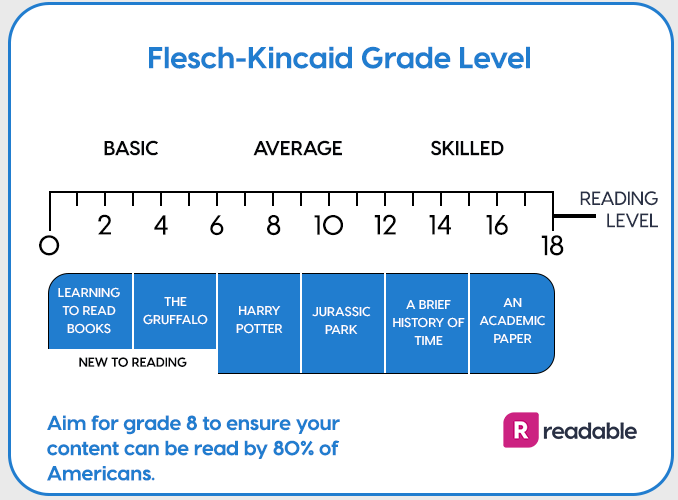
\includegraphics[width=\linewidth]{img/Screenshot_302.png}
	\caption{Bron van \textcite{Readable2021}}
\end{figure}


% https://readable.com/readability/flesch-reading-ease-flesch-kincaid-grade-level/

% Bovendien zijn er kant-en-klare modellen die de complexiteit van tekst kunnen bepalen, hoewel deze beperkt zijn en vooral gericht zijn op Engelse teksten, zoals BERT\footnote{https://huggingface.co/docs/transformers/model\_doc/bert}, XLNet\footnote{https://huggingface.co/docs/transformers/model\_doc/xlnet}, GPT-3\footnote{https://platform.openai.com/docs/} en een open-source model genaamd TRUNAJOD\footnote{https://trunajod20.readthedocs.io/}.

%---------- Methodologie ------------------------------------------------------
\section{Methodologie}%
\label{sec:methodologie}

% wat is tekstsimplificatie - welke soorten tekstsimplificatie 
% hoe bevoordeelt het aan scholieren met dyslexie in het derde graad secundair - wat zijn de struikelblokken
% welke software wordt er momenteel ingezet + vrij beschikbare software
% opbouw van een tekstsimplificatiepipeline + evaluatietechnieken

Het onderzoek houdt zeven fases in. De eerste fase is het proces van tekstsimplificatie beschrijven, waaronder een omschrijving van het begrip en de verschillende soorten van technologische tekstsimplificatie. Dit gebeurt via een grondige studie van vakliteratuur en wetenschappelijke teksten. Ook blogs van experten komen hier aan bod. Na het verwerven van de nodige inzichten wordt er een verklarende tekst opgesteld.

De tweede fase bestaat uit het analyseren van wetenschappelijke werken over de bewezen voordelen van tekstsimplificatie bij scholieren met dyslexie van het derde graad middelbaar onderwijs. Hiervoor zijn geringe thesissen beschikbaar, die zorgvuldigheid vragen tijdens interpretatie. De resulterende tekst bevat de voordelen samen met hun wetenschappelijke onderbouwing.

De derde fase is het verzamelen van alle nodige transformaties om een wetenschappelijke paper beter leesbaar te maken voor een scholier met dyslexie in het derde graad middelbaar onderwijs. Het resultaat is een shortlist van alle evaluatiecriteria waaraan de outputtekst van een tekstsimplificatietoepassing moet voldoen.

De vierde fase is opnieuw een beschrijving. Hier worden de valkuilen bij taalverwerking met AI-software nagegaan. Deze fase van het onderzoek brengt mogelijke nadelen en tekortkomingen van AI-software bij tekstsimplificatie aan het licht. Dit gebeurt aan de hand van een technische uitleg.

De vijfde fase omvat een toelichting en advies over de beschikbare Nederlandstalige AI-tools voor tekstsimplificatie. Aan de hand van een veldonderzoek op het internet en bij bedrijven wordt er op zoek gegaan naar dergelijke software. Er wordt niet gezocht naar vertaalsoftware of toepassingen die de inhoud van een afbeelding of tekstbestand omzet naar tekstinhoud.

De zesde fase omschrijft een shortlist van de benodigde machineleertechnieken om zelf een tekstsimplificatiepipeline op te bouwen, alsook een shortlist van metrieken om de transformatie te evalueren. Op basis van de metrieken wordt er een pipeline ontwikkeld met beschikbare kant-en-klare bibliotheken en algoritmes. Het resultaat van deze fase is een pipeline opgebouwd in de programmeertaal Python. 

De zevende en laatste fase omvat een vergelijkende studie met de gevonden applicaties en de zelfgemaakte pipeline. Wetenschappelijke papers, die in een derde graad middelbaar onderwijs worden ingezet, dienen hier als invoertekst. De transformatie wordt met zowel objectieve als subjectieve metrieken beoordeeld. De subjectieve test gebeurt aan de hand van een \textit{survey} en een \textit{think-aloudtest}. De objectieve testen gebeuren op basis van de shortlist uit de derde fase en de shortlist van metrieken uit de zesde fase. Ten slotte volgt er een persoonlijk advies over de nodige ontwikkelingen in het vak op vlak van Nederlandstalige tekstsimplificatie.

%---------- Verwachte resultaten ----------------------------------------------
\section{Verwacht resultaat, conclusie}
\label{sec:verwachte_resultaten}

Er wordt verwacht dat de software, die momenteel in het onderwijs wordt ingezet, niet voldoet aan de noden van een scholier met dyslexie in het derde graad middelbaar onderwijs. Dit is omdat er onvoldoende rekening wordt gehouden met hun unieke uitdagingen. Het vertalen van de outputtekst bij een internationale AI-tool zal mogelijk afwijken van de oorspronkelijke context. 

Er zijn onvoldoende kant-en-klare algoritmen en modellen beschikbaar om een tekstsimplificatiepipeline, waarvan de output verzorgd is aan de unieke noden van een scholier met dyslexie in het derde graad middelbaar onderwijs, te bouwen. De pipeline vergt \textit{custom transformers} om nauwkeurige resultaten te bekomen, zodat de kerninhoud niet verloren raakt. Het vertalen van de zinnen verlaagt de nauwkeurigheid van het model, maar is een acceptabel alternatief. Er is nood aan Nederlandstalige \textit{word embeddings} die de complexiteit per woord bijhouden, alsook meer kant-en-klare modellen die tekstsimplificatiefuncties aanbieden.